\documentclass[12pt]{article}

\usepackage[utf8]{inputenc}
\usepackage[margin=1in]{geometry}
\renewcommand{\baselinestretch}{1}
\usepackage{indentfirst}

\usepackage{amsmath, amssymb}

\usepackage{hyperref}
\usepackage{cleveref}
\usepackage{graphicx}
\usepackage{subfigure}
\usepackage{float}
\graphicspath{{./figs/}}

\usepackage{fancyvrb}

\usepackage{natbib}
\bibliographystyle{aasjournal}

\begin{document}

\begin{center}\begin{LARGE}
\textbf{ASTR 5900 Final Project: Hydro1D}
\end{LARGE}\end{center}

\begin{center}
\textbf{Anthony Burrow and Sarah Stangl}
\end{center}

\section{Introduction and Goals}

This project is aimed to model the infall and subsequent shockwave exhibited by
core-collapse supernovae (CCSNe). In modern studies of all types of SNe
(including Type Ia SNe, CCSNe, etc.), one of the most prominent goals is to achieve a better understanding of the so-called progenitor problem. To
briefly summarize, we wish for the ability to understand the different possible
scenarios of a supernova progenitor as well as to diagnose the scenario with
observable features from the subsequent explosion. If this could be achieved,
this would provide insight into stellar evolution as a whole and minimize a
large source of uncertainty in many interesting predictions in astronomy made
by using these SNe.

The goal of this project is only to model the dynamics of the collapse of a
massive ($\sim10\ M_\odot$) star. This is done using a 1D Lagrangian
hydrodynamical code that solves equations of mass conservation, momentum
conservation, and energy conservation, with the addition of an equation of
state. Our secondary and hopeful goal is to implement a distinguishable shock event
that should occur when a bulk of infalling material rapidly rebounds off of a
highly dense and degenerate core of neutrons. This shockwave is what signifies that a CCSN explosion occurs.

\section{Methods}

To generate the aforementioned model, we first assume a star of mass
$10\ M_\odot$ coming directly from hydrostatic equilibrium. The star's collapse
would be caused by a sudden decrease in pressure. The model is separated into a
set number of zones, all with equal mass. Because this is a Lagrangian
hydrocode, the zones always have the same constant mass.

\subsection{Initial Model}
The initial conditions (radius, density, pressure) are all solved for hydrostatic equilibrium through the Lane-Emden equation,
\begin{equation}\label{eq:laneE}
    \frac{1}{\xi^{2}}\frac{d}{d\xi}\left( \xi^{2}\frac{dD_{n}}{d\xi} \right)=-D_{n}^{n},
\end{equation}
where $\xi$ is a dimensionless independent variable related to radius,  $D_{n}(\xi)$ is a
dimensionless function related to density, and $n$ is the polytropic index. We impose the
boundary conditions
\begin{equation}
\begin{split}
    D_{n}(\xi_{1})=0, \\
    D_{n}(0) = 1, \\
    D_{n}'(0) = 0
\end{split}
\end{equation}
where $\xi_{1}$ is the first root of the solution corresponding to the star's surface \citep{bob}.

Solving \autoref{eq:laneE} for $D_{n}(\xi)$ leads directly to the density as a function of radius,
\begin{equation}
    \rho(r)=\rho_{c}[D_{n}(r)]^{n},
\end{equation}
where $\rho_{c}$ is the central density.
The radius is given by
\begin{equation}
    r = \lambda_{n} \xi,
\end{equation}
where
\begin{equation}
    \lambda_{n}=\left[(n+1)\left( \frac{K \rho_{c}^{(1-n)/n}}{4\pi G} \right) \right]^{1/2}
\end{equation}
with Newton's gravitational constant $G$, and a constant $K$.
% \iffalse
% \begin{equation}
%     K = \left[ \frac{3(1-\beta}{a}\right]^{1/3}\left(\frac{k}{\beta \mu m_{H}} \right)^{4/3}
% \end{equation}
% \fi
The mass enclosed at each radius is calculated from
\begin{equation}
    M_{int}(r) = -4 \pi \lambda_{n}^{3} \rho_{c} \left.\left(\xi^2 \frac{dD}{d\xi}\right)\right|_{\xi=\xi_1}.
\end{equation}

We assume the polytropic equation of state of
$P = K_{4/3}\ \rho^{4/3}$, where $P$ is outward gas pressure. $K$ can be found
by integrating total mass,
\begin{equation}
    M = \int_0^R 4\pi r^2 \rho dr = 4\pi \lambda^3 \rho_c \int_0^{\xi_1} \xi^2 D^n d\xi,
\end{equation}
and solving for $K = K_{4/3}$ using \autoref{eq:laneE} for $n=3$ yields
\begin{equation}
    K_{4/3} = \pi G \left[ \frac{M}{4\pi} \left.\left(-\xi^2 \frac{dD}{d\xi}\right)\right|_{\xi=\xi_1} \right]^{2/3} \approx 1.784 \times 10^{15}\ [\text{cgs}],
\end{equation}
for $M = 10\ M_\odot$ and is independent of $\rho_c$. This equation of state is for densities under nuclear degeneracy
$\rho_{nuc} = 2.3 \times 10^{14}$ g cm$^{-3}$. We also assume an initial
central density of $\rho_c = 1.0 \times 10^7$ g cm$^{-3}$.

\begin{figure}[ht]
    \centering
    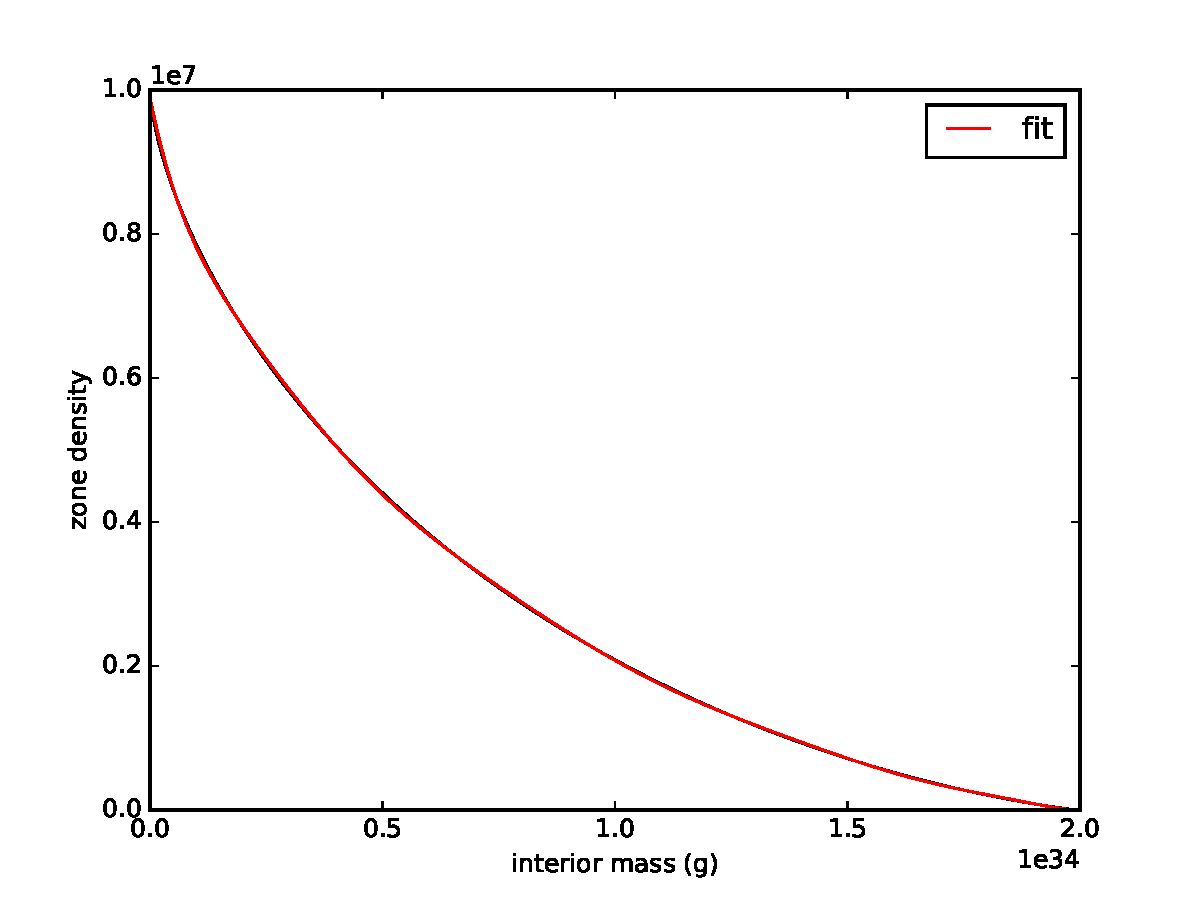
\includegraphics[width=0.7\textwidth]{rho_mass}
    \caption{Calculated density versus interior mass throughout the star. The red line
             shows a polynomial fit to the calculation, and was used to interpolate
             density for the hydrocode input.}
    \label{fig:rho_mass}
\end{figure}

\autoref{fig:rho_mass} shows a plot of calculated $\rho$ as a function of interior
mass throughout the stellar model. We fit a $10^\text{th}$ order polynomial to this
calculation to interpolate the density for any given number of zones that the user wishes to
model. This interpolation was done such that each zone was of equal mass and was given
to the hydrocode as input.


\subsection{Hydrodynamical Calculations}

Once these initial conditions have been set, the dynamics of density, pressure,
and velocities are calculated by following the exact difference equations found
in the Appendix of \citet{arnett66}. However, because of time constraints, we
simplify the calculation heavily by not accounting for radiation or neutrinos
as a source or sink of energy. Because we assume a polytropic equation of state, our
model also has zero temperature, and no temperature calculations are needed.
We create our model with 100 zones, and the hydrocode evaluates many properties
of these zones as a function of time.
From the initial conditions, we do 10,000 iterations of calculating zone
boundary velocities ($U_j$), boundary positions ($R_j$), specific volume of
each zone ($V_{j + 1/2} = 1 / \rho_{j + 1/2}$), and zone pressure
($P_{j + 1/2}$) in that order. These are calculated using basic Eulerian difference
equations that describe the equations of mass, momentum, and energy
conservation, and they are all listed in the Appendix of \citet{arnett66}.

From an initial time step (we typically us $\Delta t^0 = 0.001$ second), each
iteration calculates a new maximum time step that holds causality due to sound
velocity. This is done in the same way as \citet{colgatewhite64} by finding the
maximum value (across all zones $j$) of
$$
\begin{aligned}
\Delta t^{n + 1/2}
&= \frac{0.02 \cdot V^n_{j + 1/2} \Delta t^{n - 1/2}}
        {|V^n_{j + 1/2} - V^n_{j - 1/2}|}, \\
\Delta t^n
&= \frac{1}{2} (\Delta t^{n + 1/2} + \Delta t^{n - 1/2}).
\end{aligned}
$$
We found that this keeps causality well for our purposes; in other words, this
means no negative densities, etc. appear due to over-correction to the
boundary positions.

To reiterate, the pressure we assume is due solely to electron pressure, i.e.
$$
\begin{aligned}
P_j = P(e^-)_j = K_{4/3}\ (1 / V_j)^{4/3}.
\end{aligned}
$$
However, to model neutron degeneracy pressure, for any zone with densities
above nuclear density $\rho_{nuc}$, this pressure is amended to
$$
\begin{aligned}
P_j = P(e^-)_j + K_3\ (1 / V_j)^3,
\end{aligned}
$$
where
$$
\begin{aligned}
K_3 = \frac{K_0}{27 \rho_c^2 m_n}
\end{aligned}
$$
with $K_0 = 140$ MeV and $m_n = 1.674920 \times 10^{-24}$ g is the mass of a
neutron. This is based on the cold nuclear pressure suggested by \citet{bck85} with
$K_0 = K_0(0.33)$ and $\gamma = 3$.

Finally, to cause a collapse, we attempt to calculate our initial hydrostatic condition
with $K'_{4/3} = 1.1 \cdot K_{4/3}$ within the equation of state, and then
lower the pressure by using $K_{4/3}$ in our subsequent iterations instead. The
lowered pressure should lead to gravitational domination and a collapse.


\section{Results}


\autoref{fig:P_rho} describes the pressure and density of a single zone ($j=5$, near the core)
in our model as it evolves in time. Clearly the polytropic equation of state is represented as a linear
trend in this log-log space. However, once the zone becomes compressed past nuclear density,
the neutron degeneracy pressure increases the total pressure substantially, which helps the
core resist collapse.

\begin{figure}[ht]
    \centering
    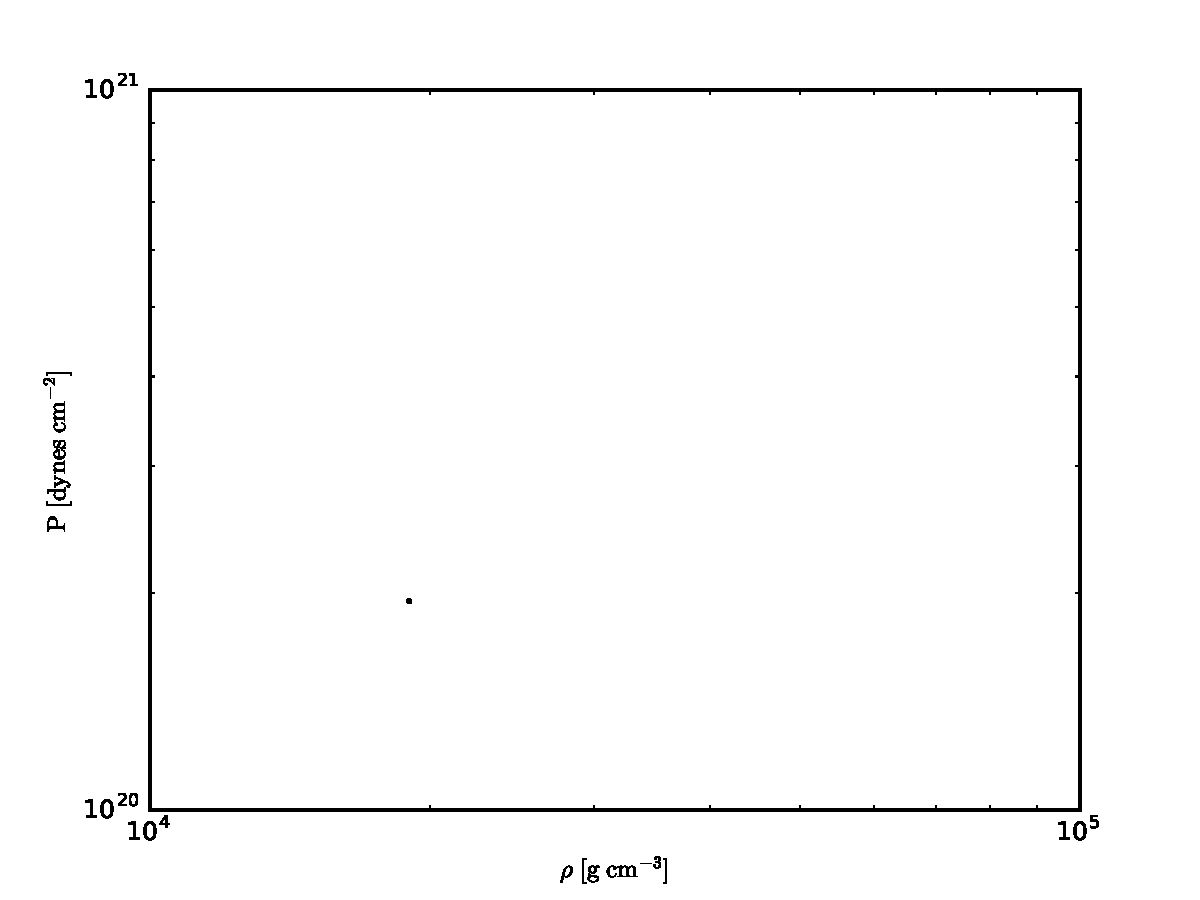
\includegraphics[width=0.7\textwidth]{P_rho}
    \caption{Pressure versus density for the $5^\text{th}$ zone from the inside (near the core).
             Each point represents an instance in time. The expected equation of state trend is
             found as the star compresses until the zone reaches nuclear densities on order of
             $10^{14}$--$10^{16}$ g cm$^{-3}$.}
    \label{fig:P_rho}
\end{figure}

Before attempting to force collapse by altering $K_{4/3}$ in the initial conditions, we wanted to
test the hydrostatic nature of the initial conditions.
In \autoref{fig:R_time}, which shows the inner boundary location of the same zone as a function of time,
it can be seen that the star ultimately becomes the most unstable against collapse at around 3.8 seconds.
Not only this, but immediately after the first iteration the star increases in size dramatically.
This is illustrative that the program did not work as intended, as our solution to the hydrostatic
Lane-Emden equation does not support itself against collapse with a polytropic equation of state.

\begin{figure}[ht]
    \centering
    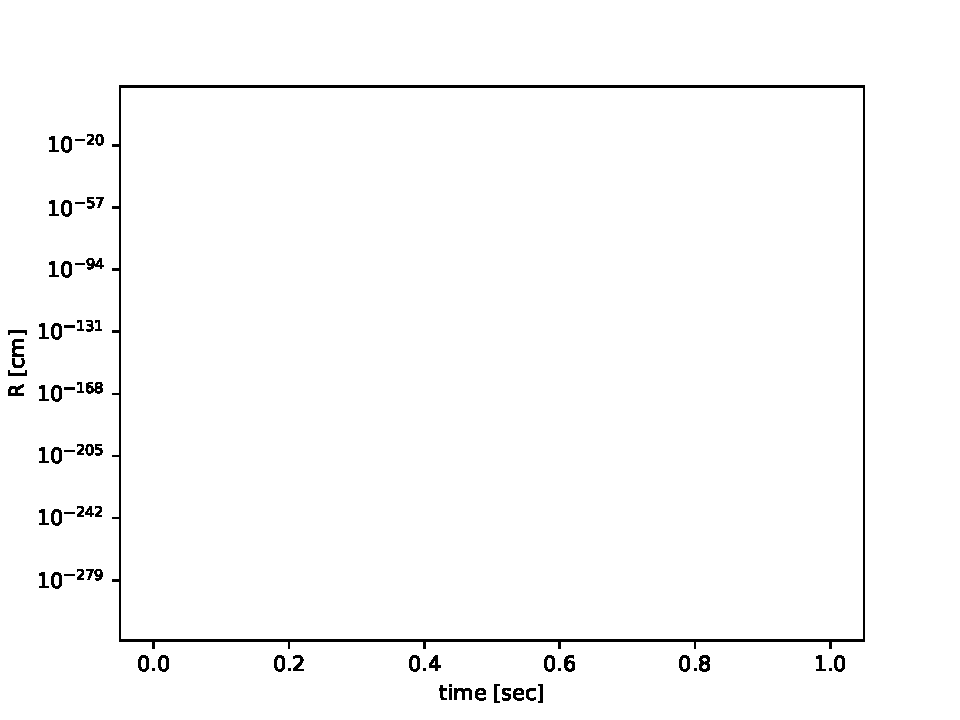
\includegraphics[width=0.7\textwidth]{R_time}
    \caption{Inner boundary position of the same zone as in \autoref{fig:P_rho} as a function of time.}
    \label{fig:R_time}
\end{figure}

To further explore the problems we had with this, we show the velocity of each zone in \autoref{fig:UR}
at six different points in time. Note the different x- and y-axis ranges at each time. In the top-left
panel, which occurs soon after initialization, we see
the outward trajectory of material throughout the star. In the next four panels (in chronological order:
top-right, middle-left, middle-right, and bottom-left) we see the star begin to quickly slow down and
begin to infall at around 1.0 second. This continues until the star is rapidly accelerating inward. However,
looking at the final (bottom-right) panel, we see what looks like the bulk of the stellar material hitting
a now extremely degenerate core, material begins to vary in velocity wildly, and near the core a spike
of outward velocity is seen. This is possibly some sort of rebound or perhaps a start of a shock event.

\begin{figure}[ht!]
    \centering
    \begin{minipage}{0.49\linewidth}
        \centering
        \begin{subfigure}{\linewidth}
            \centering
            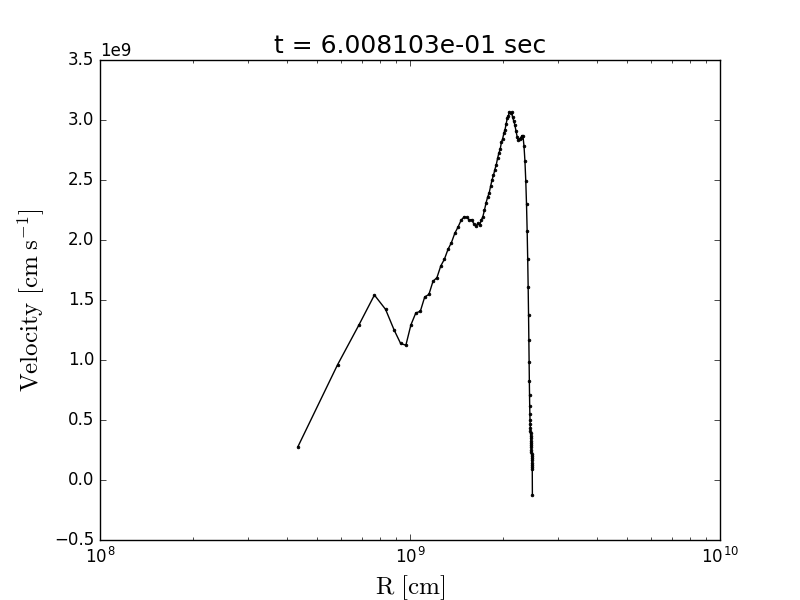
\includegraphics[width=\linewidth]{figs/U_R_6.008103e-01.png}
        \end{subfigure}
        \begin{subfigure}{\linewidth}
            \centering
            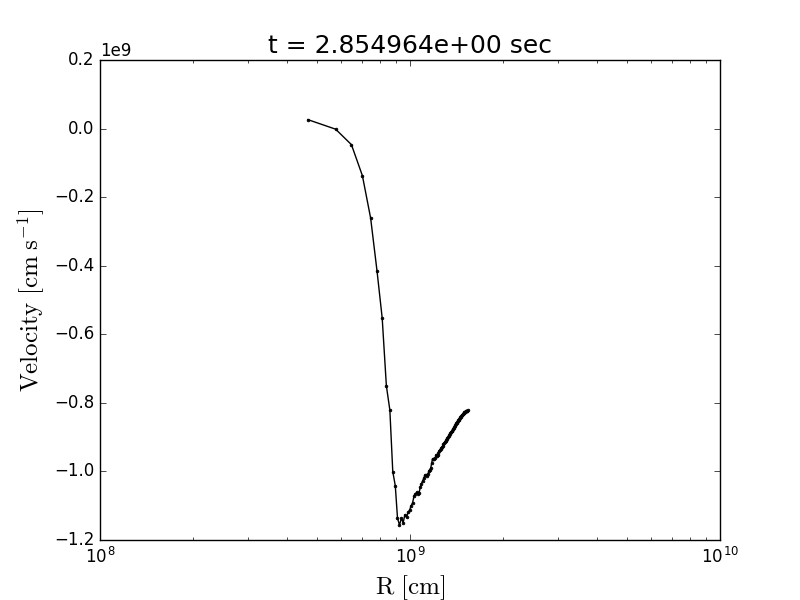
\includegraphics[width=\linewidth]{figs/U_R_2.854964e+00.png}
        \end{subfigure}
        \begin{subfigure}{\linewidth}
            \centering
            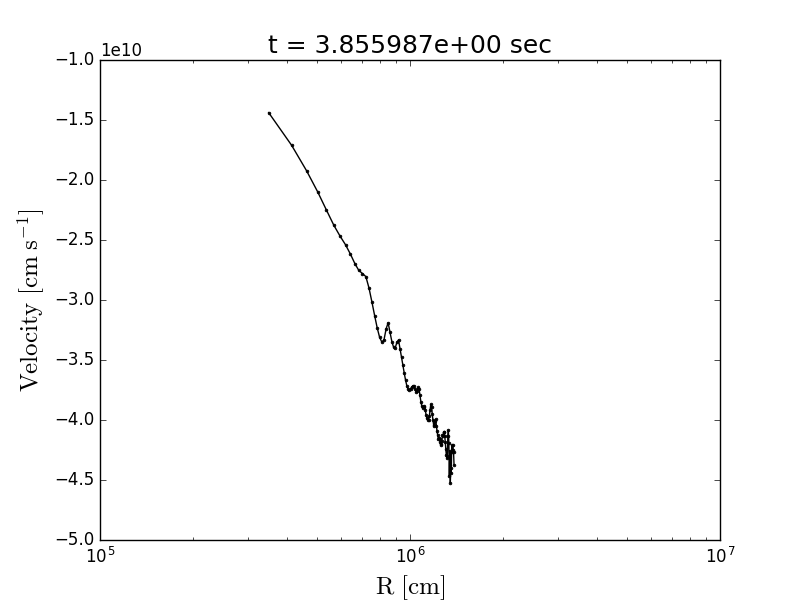
\includegraphics[width=\linewidth]{figs/U_R_3.855987e+00.png}
        \end{subfigure}
    \end{minipage}
    \hfill
    \begin{minipage}{0.49\linewidth}
        \centering
        \begin{subfigure}{\linewidth}
            \centering
            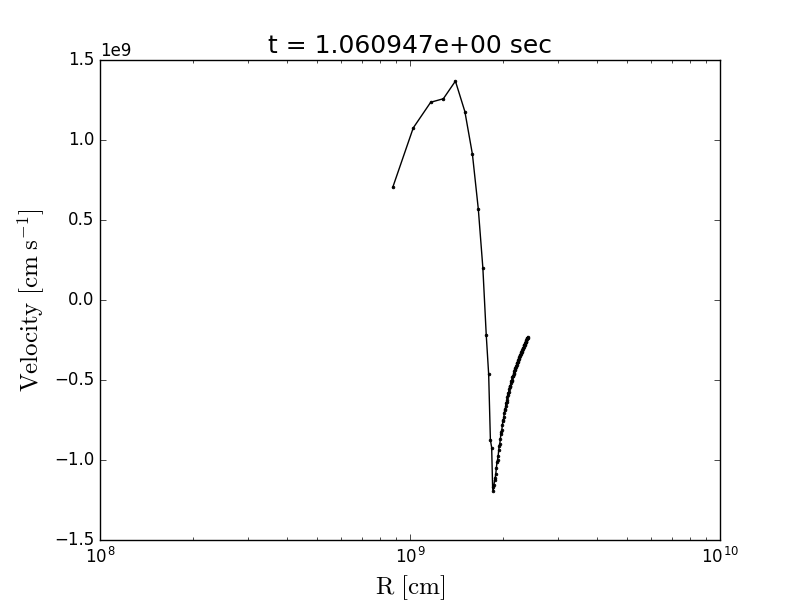
\includegraphics[width=\linewidth]{figs/U_R_1.060947e+00.png}
        \end{subfigure}
        \begin{subfigure}{\linewidth}
            \centering
            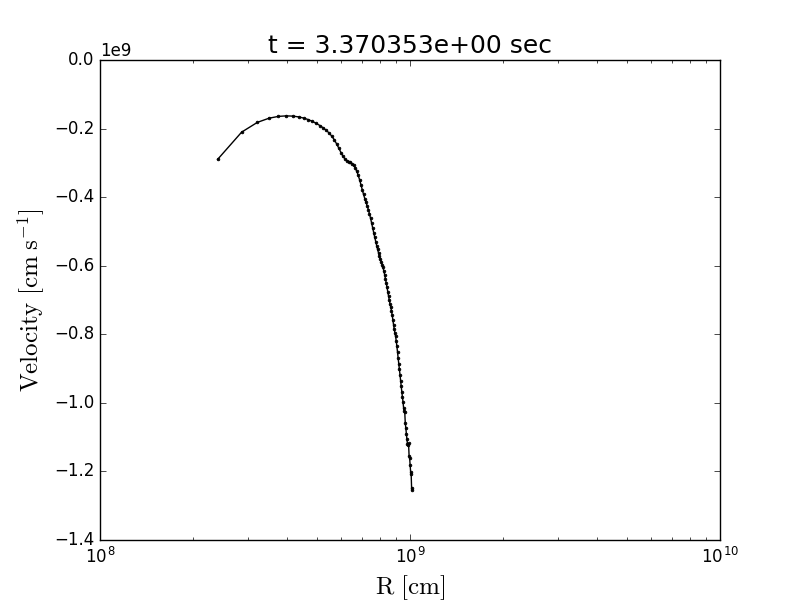
\includegraphics[width=\linewidth]{figs/U_R_3.370353e+00.png}
        \end{subfigure}
        \begin{subfigure}{\linewidth}
            \centering
            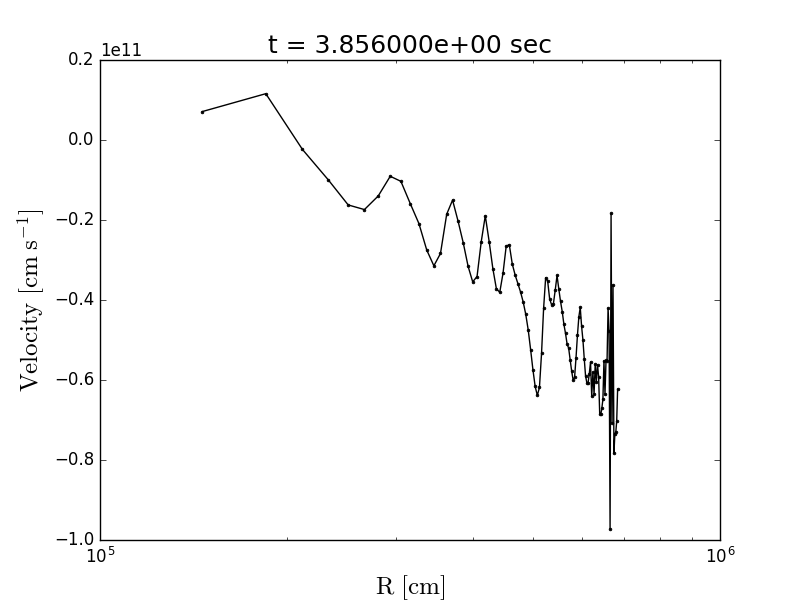
\includegraphics[width=\linewidth]{figs/U_R_3.856000e+00.png}
        \end{subfigure}
    \end{minipage}
    \caption{Boundary velocity versus position for each zone, represented as points. Each panel
             shows a different point in time throughout the model's evolution; time progresses
             from left to right, top to bottom, and the time is displayed above each panel.}
    \label{fig:UR}
\end{figure}


\section{Discussion and Conclusion}

It is clear that the work in this project does not accurately portray the true dynamics of
a star. Our first test of this hydrocode was to ensure that the model is stable upon receiving
hydrostatic initial conditions, and clearly it failed to do so. Our primary reasoning as to why
the model was unstable (aside from just a "bug in the code") is that the initial conditions
may not be as precise as needed for the differential treatment of solving the equations.
If this is the case, it could be an interpolation error in going between the hydrostatic solution
to the hydrocode input.

It could also be that there could be a mistake in translating a
density-versus-interior mass interpolation into boundary positions for each zone. This process
involves a subtraction that could have led to a loss in precision. We may also need to
perform some sort of density integration to go from mass to radial space, which was not
done in our method. Regardless, one of these
reasons is a likely scenario that could cause the model to immediately begin to rapidly
expand, and the limitations of the simple difference equations within the hydrocode could
not correctly capture the behavior of the star.

If we had more time, or if this project were to continue, the next step in attempting to fix
our unstable model would be to look closely at the interpolation, as well as how the boundary
positions are calculated. This project was a great illustration of the importance
of precise initial conditions.


\appendix
\begin{center}\begin{LARGE}
\textbf{Appendix}
\end{LARGE}\end{center}


\section{Division of Work}

Anthony created the structure and setup the underlying mathematical equations within the hydrocode
itself. He also assisted in connecting the initial conditions from Sarah to the input of
the hydrocode.

Sarah worked on solving the Lane-Emden equation and deriving the initial model conditions from the results. She also attempted to help get the hydrocode working using physics she'd used in hydrocodes in the past. Also, she tried playing around with model parameters and the K value to try, unsuccessfully, to get a shock.

We both worked on writing the final paper.


\section{Running the Program}

The full details of how to compile and run the program are provided in the README document of the attached
codebase\footnote{see also https://github.com/anthonyburrow/Hydro1D/} that is also at the end of this
document. This section is mainly provided to ensure and prove that we did create a compilable and running code.

The program may be fully compiled below in the following way:
\begin{figure}[H]
    \centering
    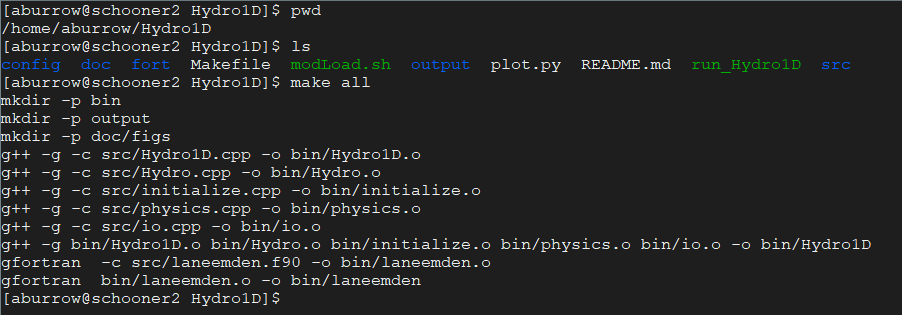
\includegraphics[width=0.95\textwidth]{compile}
    \label{fig:compile}
\end{figure}
When running the full program, the terminal output describes each step of the process:
\begin{figure}[H]
    \centering
    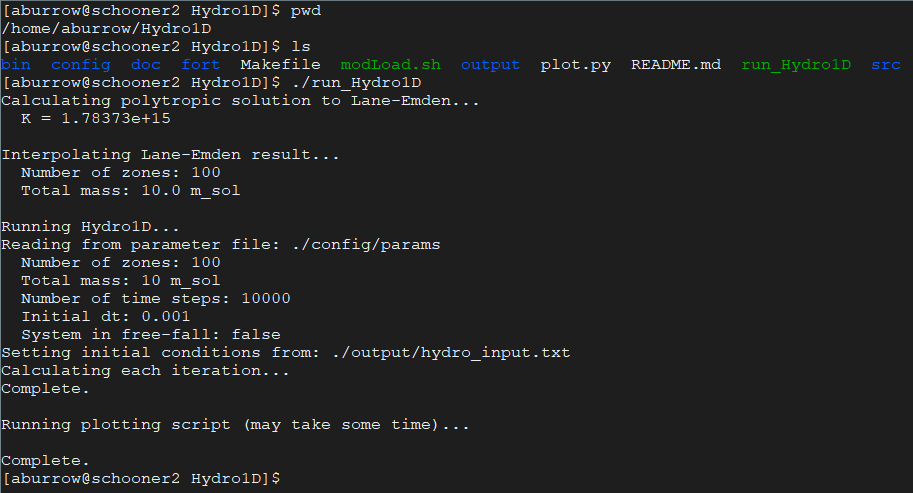
\includegraphics[width=0.95\textwidth]{run}
    \label{fig:run}
\end{figure}

This program generates a few human-readable data files in an \texttt{output/} directory within the
root directory. These output data files are then plotted and are the plots seen in the above figures.

\bibliography{bib}

\pagebreak

The scripts and implementation files of our source code is given below:

\texttt{laneemden.f90}
\begin{Verbatim}[fontsize=\small]
program laneem
! code taken from http://www.astro.utu.fi/~cflynn/Stars/l4.html
        use, intrinsic :: iso_fortran_env
        implicit none

        real x, dxdt, n, dt, xlast, dxdtlast, t
        integer i
        character*50 name


        ! write(6,*) 'Enter n, the polytrope index '
        ! read(5,*) n

        n = 3

        if (n.ge.5) then
          write(6,*) 'n is too big, star radius is infinite'
          stop
        end if

        ! write(6,*) 'Enter name of results file'
        ! read(5,*) name

        name = './output/poly3'

        open(20,file=name,status='new')


        x    = 1.0
        dxdt = 0.0
        t    = 0.0001


        dt = 0.001


        do 100 i = 1, 10000

          dxdt = dxdt - ( 2.0*dxdt/t + x**n )*dt

          x = x + dxdt*dt

          t = t + dt


          write(20,*) t,x,dxdt

          if (x.lt.0.0) goto 999

100     continue

999     continue

        end
\end{Verbatim}

\pagebreak
\texttt{fileToIP.py}
\begin{Verbatim}[fontsize=\small]
import numpy as np


# read in the results from the lane-emden calculations
#   xi    -- dimensionless parameter used in Caroll and Ostille
#   D     -- dimensionless parameter used in Caroll and Ostille
#   dDdXI -- change in D
data = np.loadtxt('./output/poly3')[:-1]

xi = data[:, 0]
D = data[:, 1]
dDdXI = data[:, 2]

n = 3
G = 6.6743e-8
msol = 1.989e33

# Read total mass
fn = './config/params'
with open(fn) as F:
    lines = F.read().splitlines()

lines = [l for l in lines if l]
lines = [np.float64(l) for l in lines if l[0] != '#']

M = lines[1] * msol

# central density, assume 10^7
rho_c = 1e7

# Calculate constant K for given total mass M
K = M / (-4 * np.pi * xi[-1]**2 * dDdXI[-1])
K = K**(2 / 3)
K *= 4 * np.pi * G / (n + 1)
print('  K = %.5e' % K)

# lambda from Caroll and Ostille, lambda = sqrt((n+1)Krho_c^((1-n)/n)/(4 pi G))
# lamb = 1.98874e8
lamb = np.sqrt((n + 1) * K * rho_c**((1 - n) / n) / (4 * np.pi * G))

# density, rho = rho_c * D^3
rho = rho_c * D**3

# pressure P = K rho^((n+1)/n)
P = K * rho**((n + 1) / n)

# radius r = lambda * xi
rad = lamb * xi

# mass enclosed -- M = 4 pi lambda^3 rho_c int_{0}^{xi}(xi'^2 * D^n dxi')
#M = (4 * 3.141592 * lamb**3 * xi**3 * D**3) / 3

# no cell centering
#fout = open('full_data.txt','w')

#fout.write('mass_enclosed, radius, density, pressure\n')

#for i in list(range(len(rho))):
#   fout.write(str(M[i])+' '+str(rad[i])+' '+str(rho[i])+' '+str(P[i])+'\n')

#fout.close()

# attempt to center cell
#fout = open('data.txt','w')

#fout.write('mass, radius, density, pressure\n')

#for i in list(range(len(rho)-1)):
#   fout.write(str(M[i+1] - M[i])+' '+str((rad[i+1]+rad[i])/2)+' '+str((rho[i+1]+rho[i])/2)+' '+str((P[i+1]+P[i])/2)+'\n')

#fout.close()

M = -4 * np.pi * lamb**3 * rho_c * xi**2 * dDdXI

fout = open('./output/data_cell_centered.txt', 'w')
fout.write('mass, radius, density, pressure\n')

for i in list(range(len(rho)-1)):
        fout.write(str(M[i])+' '+str((rad[i+1]+rad[i])/2)+' '+str((rho[i+1]+rho[i])/2)+' '+str((P[i+1]+P[i])/2)+'\n')

fout.close()
\end{Verbatim}

\pagebreak
\texttt{interpolate.py}
\begin{Verbatim}[fontsize=\small]
import numpy as np
import matplotlib.pyplot as plt
plt.switch_backend('agg')


msol = 1.989e33
rhoc = 1e7


# Read Lane-Emden output
fn = './output/data_cell_centered.txt'
data = np.loadtxt(fn, skiprows=1)

data = data[:data[:, 0].argmax() + 1]   # correct for decreasing int. mass

m_int = data[:, 0]
radius = data[:, 1]
density = data[:, 2]

# Read parameters
fn = './config/params'
with open(fn) as F:
    lines = F.read().splitlines()

lines = [l for l in lines if l]
lines = [np.float64(l) for l in lines if l[0] != '#']

n_zones = int(lines[0])
n_boundaries = n_zones + 1
total_mass = lines[1] * msol
dm = total_mass / n_zones

print('  Number of zones: %i' % n_zones)
print('  Total mass: %.1f m_sol' % lines[1])

# Fit output
params = np.polyfit(m_int / total_mass, density / rhoc, 10)
poly = np.poly1d(params)

m_predict = np.linspace(1e-70 / total_mass, 1, n_boundaries)

output = np.zeros((n_zones, 3))
output[:, 0] = m_predict[1:] * total_mass
output[:, 2] = poly((m_predict[1:] + m_predict[:-1]) / 2) * rhoc

prev_R_cube = 0
pi4_3 = 4 * np.pi / 3
for i in range(n_zones):
    new_R_cube = prev_R_cube + dm / (output[i, 2] * pi4_3)
    output[i, 1] = np.cbrt(new_R_cube)

    prev_R_cube = new_R_cube

fn = './output/hydro_input.txt'
np.savetxt(fn, output, fmt=['%.12e', '%.12e', '%.12e'])

# Plot fit
fig, ax = plt.subplots(dpi=200)

ax.plot(m_int, density, 'ko', ms=0.5)
ax.plot(m_predict * total_mass, poly(m_predict) * rhoc, 'r-', label='fit')

ax.set_xlabel('interior mass (g)')
ax.set_ylabel('zone density')

ax.set_xlim(left=0)
ax.set_ylim(0, rhoc)

ax.legend()

fn = './doc/figs/rho_mass.pdf'
fig.savefig(fn, dpi=200)
\end{Verbatim}

\pagebreak
\texttt{Hydro1D.cpp}
\begin{Verbatim}[fontsize=\small]
#include <iostream>

#include "io.hpp"
#include "Hydro.hpp"

using namespace std;

int main(int argc, char* argv[])
{
    myHydro::hydroParams params = myHydro::readParams();
    myHydro::Hydro hydro(params);

    hydro.write();

    cout << "Calculating each iteration..." << endl ;
    while (hydro.iter < hydro.nIter)
    {
        hydro.iterate();
        hydro.write();
    }

    cout << "Complete." << endl;

    return 0;
}
\end{Verbatim}

\pagebreak
\texttt{Hydro.cpp}
\begin{Verbatim}[fontsize=\small]
#include <iostream>
#include <string>

#include "Hydro.hpp"

#include "io.hpp"
#include "initialize.hpp"
#include "physics.hpp"
#include "constants.hpp"

using namespace std;

namespace myHydro
{
    Hydro::Hydro(const myHydro::hydroParams &params)
      : // Allocate vectors
        U(params.nZones + 1),
        R(params.nZones + 1),
        Rht(params.nZones + 1),
        V(params.nZones),
        Vprev(params.nZones),
        Vht(params.nZones),
        XM(params.nZones + 1),
        Q(params.nZones),
        Pht(params.nZones),
        Tht(params.nZones),
        ET(params.nZones),
        EV(params.nZones),
        T(params.nZones),
        P(params.nZones),

        // Output
        filedt("./output/dt.dat"),
        fileU("./output/U.dat"),
        fileR("./output/R.dat"),
        fileV("./output/V.dat"),
        // fileT("./output/T.dat"),
        fileP("./output/P.dat"),
        fileQ("./output/Q.dat")
    {
        // Parameters
        nZones = params.nZones;
        nBoundaries = nZones + 1;
        nIter = params.nIter;
        totalMass = params.totalMass * myHydro::msol;
        freeFall = params.freeFall;

        iter = 0;

        dt = params.initDt;
        dtht = params.initDt;   // half-time time interval

        // Adjust output
        myHydro::setOutputPrecision(*this);

        // Setup
        initVectors();
    }

    void Hydro::initVectors()
    {
        myHydro::readHydrostatic(*this);

        myHydro::calcDM(*this);

        myHydro::initU(*this);

        myHydro::calcXM(*this);   // can either read or calculate

        myHydro::initQ(*this);
        myHydro::initT(*this);
        myHydro::calcP(*this);
    }

    void Hydro::iterate()
    {
        myHydro::calcU(*this);
        myHydro::calcR(*this);
        myHydro::calcV(*this);

        myHydro::calcQ(*this);
        myHydro::calcPht(*this);
        myHydro::calcET(*this);
        myHydro::calcEV(*this);

        // myHydro::calcT(*this);
        myHydro::calcP(*this);

        myHydro::calcDt(*this);

        iter++;
    }

    void Hydro::write()
    {
        myHydro::writeOutput(*this);
    }
}
\end{Verbatim}

\pagebreak
\texttt{initialize.cpp}
\begin{Verbatim}[fontsize=\small]
#include <iostream>
#include <vector>
#include <cmath>

#include "Hydro.hpp"
#include "constants.hpp"
#include "io.hpp"

using namespace std;

namespace myHydro
{
    void initU(myHydro::Hydro &hydro)
    {
        hydro.U[0] = myHydro::zero;   // BC

        // Start from rest
        for (int i = 1; i < hydro.nBoundaries; i++)
        {
            hydro.U[i] = myHydro::zero;
        }
    }

    void initQ(myHydro::Hydro &hydro)
    {
        // No pseudoviscosity at the start
        for (int i = 0; i < hydro.nZones; i++)
        {
            hydro.Q[i] = myHydro::zero;
        }
    }

    void initT(myHydro::Hydro &hydro)
    {
        // initial temperature profile
        for (int i = 0; i < hydro.nZones; i++)
        {
            hydro.T[i] = myHydro::zero;
        }

        hydro.Tht = hydro.T;   // Initial assumption
    }

}
\end{Verbatim}

\pagebreak
\texttt{physics.cpp}
\begin{Verbatim}[fontsize=\small]
#include <vector>
#include <cmath>
#include <iostream>

#include <iomanip>

#include "Hydro.hpp"
#include "physics.hpp"
#include "constants.hpp"

using namespace std;

namespace myHydro
{
    void calcDM(myHydro::Hydro &hydro)
    {
        // Uniform mass per zone
        hydro.DM = hydro.totalMass / hydro.nZones;
    }

    void calcXM(myHydro::Hydro &hydro)
    {
        hydro.XM[0] = myHydro::zero;   // BC

        for (int i = 0; i < hydro.nZones; i++)
        {
            hydro.XM[i + 1] = hydro.XM[i] + hydro.DM;
        }
        // cout << hydro.XM[hydro.nZones] / 1.989e33 << " m_sol" << endl;
    }

    void calcR(myHydro::Hydro &hydro)
    {
        double newR;

        for (int i = 1; i < hydro.nBoundaries; i++)
        {
            newR = hydro.R[i] + hydro.U[i] * hydro.dtht;

            hydro.Rht[i] = 0.5 * (hydro.R[i] + newR);

            hydro.R[i] = newR;
        }
    }

    void calcU(myHydro::Hydro &hydro)
    {
        double R_sq;
        double dP;
        double dQ;
        const int &nZones = hydro.nZones;

        for (int i = 1; i < nZones; i++)
        {
            R_sq = pow(hydro.R[i], 2);
            dP = hydro.P[i] - hydro.P[i - 1];   // P at each boundary
            dQ = hydro.Q[i] - hydro.Q[i - 1];   // Q at each boundary

            hydro.U[i] = hydro.U[i] -
                         hydro.dt *
                             (myHydro::pi4_sq * R_sq * (dP + dQ) / hydro.DM
                             + myHydro::G * hydro.XM[i] / R_sq);
        }

        // Outer boundary with dP = dQ = 0
        R_sq = pow(hydro.R[nZones], 2);
        hydro.U[nZones] = hydro.U[nZones] -
                          hydro.dt * myHydro::G * hydro.XM[nZones] / R_sq;
    }

    void calcV(myHydro::Hydro &hydro)
    {
        double RCube = myHydro::zero;
        double nextRCube;

        for (int i = 0; i < hydro.nZones; i++)
        {
            hydro.Vprev[i] = hydro.V[i];

            nextRCube = pow(hydro.R[i + 1], 3);
            hydro.V[i] = myHydro::pi4_3 * (nextRCube - RCube) / hydro.DM;
            RCube = nextRCube;

            hydro.Vht[i] = 0.5 * (hydro.V[i] + hydro.Vprev[i]);
        }
    }

    void calcQ(myHydro::Hydro &hydro)
    {
        double dU;

        for (int i = 0; i < hydro.nZones; i++)
        {
            dU = hydro.U[i + 1] - hydro.U[i];

            if (hydro.V[i] < hydro.Vprev[i] && dU < 0)
            {
                hydro.Q[i] = 2.0 * pow(dU, 2) / hydro.Vht[i];
            }
            else { hydro.Q[i] = myHydro::zero; }

        }
    }

    void calcPht(myHydro::Hydro &hydro)
    {
        for (int i = 0; i < hydro.nZones; i++)
        {
            if (hydro.freeFall)
            {
                hydro.Pht[i] = myHydro::zero;
            }
            else
            {
                polytropicEoS(hydro.Pht[i], hydro.Tht[i], hydro.Vht[i]);
            }
        }
    }

    void calcET(myHydro::Hydro &hydro)
    {
        // ETht as a function of Tht, Vht
        for (int i = 0; i < hydro.nZones; i++)
        {
            hydro.ET[i] = myHydro::zero;
        }
    }

    void calcEV(myHydro::Hydro &hydro)
    {
        // EVht as a function of Tht, Vht
        for (int i = 0; i < hydro.nZones; i++)
        {
            hydro.EV[i] = myHydro::zero;
        }
    }

    void calcT(myHydro::Hydro &hydro)
    {
        double prevT;

        for (int i = 0; i < hydro.nZones; i++)
        {
            // // Calc T
            prevT = hydro.T[i];

            hydro.T[i] = hydro.T[i]
                         // Hydro terms
                         - (hydro.V[i] - hydro.Vprev[i])
                               * (hydro.P[i] + hydro.Q[i] + hydro.EV[i])
                               / hydro.ET[i];

            // Calc Tht
            hydro.Tht[i] = 1.5 * hydro.T[i] - 0.5 * prevT;
        }
    }

    void calcP(myHydro::Hydro &hydro)
    {
        for (int i = 0; i < hydro.nZones; i++)
        {
            if (hydro.freeFall)
            {
                hydro.P[i] = myHydro::zero;
            }
            else
            {
                polytropicEoS(hydro.P[i], hydro.T[i], hydro.V[i]);
            }
        }
    }

    void polytropicEoS(double &P, const double &T, const double &V)
    {
        const double rho = 1 / V;

        // Assume star made up of relativistic fermions (gamma = 4/3)
        const double Pelectron = myHydro::K4_3 * pow(rho, myHydro::four_thirds);

        if (rho < myHydro::rhoNuc)
        {
            // Only electron degeneracy
            P = Pelectron;
        }
        else
        {
            // Assume "stiff" gamma = 3 for nuclear degeneracy, plus the
            //    electron degeneracy term
            P = Pelectron + myHydro::K3 * pow(rho, 3.0);
        }
    }

    void calcDt(myHydro::Hydro &hydro)
    {
        // Update dt for stability
        double newDtht = myHydro::zero;
        double tmpDt;

        for (int i = 0; i < hydro.nZones; i++)
        {
            tmpDt = 0.02 * hydro.V[i] * hydro.dtht /
                        abs(hydro.V[i] - hydro.Vprev[i]);

            if (i == 0 || tmpDt < newDtht) { newDtht = tmpDt; }
        }

        hydro.dt = 0.5 * (hydro.dtht + newDtht);
        hydro.dthtPrev = hydro.dtht;
        hydro.dtht = newDtht;
    }
}
\end{Verbatim}

\pagebreak
\texttt{constants.hpp}
\begin{Verbatim}[fontsize=\small]
#pragma once

#define _USE_MATH_DEFINES
#include <cmath>

namespace myHydro
{
    // Math constants
    static const double zero = 1e-70;
    static const double pi4 = 4.0 * M_PI;
    static const double pi4_sq = pi4 * pi4;
    static const double one_third = 1.0 / 3.0;
    static const double four_thirds = 4.0 / 3.0;
    static const double pi4_3 = pi4 * one_third;

    // Units
    static const double msol = 1.989e33;   // Solar mass (g)

    // Newton gravitation constant
    static const double G = 6.6743e-8;   // Dyne cm g

    // Nuclear density
    static const double rhoNuc = 2.3e14;   // g cm^-3

    // Polytropic (gamma = 4/3) pressure constant for 10 m_sol
    // static const double K4_3 = 1.2e15;   // cgs
    static const double K4_3 = 1.78373175076e15;   // cgs

    // Polytropic (gamma = 2) pressure constant
    //    Based on Baron, Cooperstein, Kahana 1985 with x = 0.33, gamma = 3
    //    P = [ K0 / (9 * gamma * rhoNuc^2 * m_n) ] * rho^3
    const double m_n = 1.674920e-24;   // Mass of neutron (g)
    const double K0 = 140.0 * 1.60218e-6;   // erg
    const double gamma = 3.0;

    static const double K3 = K0 / (9.0 * gamma * pow(rhoNuc, 2.0) * m_n);
}
\end{Verbatim}

\pagebreak
\texttt{io.cpp}
\begin{Verbatim}[fontsize=\small]
#include <iostream>
#include <string>
#include <fstream>
#include <sstream>
#include <limits>
#include <iomanip>

#include "io.hpp"
#include "Hydro.hpp"
#include "constants.hpp"

using namespace std;

namespace myHydro
{
    myHydro::hydroParams readParams()
    {
        string filename = "./config/params";
        cout << "Reading from parameter file: " << filename << endl;

        ifstream paramFile(filename);
        string line;
        myHydro::hydroParams params;

        int count = 0;
        while (getline(paramFile, line))
        {
            if (line[0] == '#' || line[0] == '\0') { continue; }

            stringstream iss(line);

            switch(count)
            {
                case 0 :
                    int nZones;
                    iss >> nZones;
                    params.nZones = nZones;
                    cout << "  Number of zones: " << nZones << endl;
                    break;
                case 1 :
                    double totalMass;
                    iss >> totalMass;
                    params.totalMass = totalMass;
                    cout << "  Total mass: " << totalMass << " m_sol" << endl;
                    break;
                case 2 :
                    double nIter;
                    iss >> nIter;
                    params.nIter = nIter;
                    cout << "  Number of time steps: " << nIter << endl;
                    break;
                case 3 :
                    double initDt;
                    iss >> initDt;
                    params.initDt = initDt;
                    cout << "  Initial dt: " << initDt << endl;
                    break;
                case 4 :
                    bool freeFall;
                    iss >> freeFall;
                    params.freeFall = freeFall;
                    cout << "  System in free-fall: ";
                    cout << boolalpha << freeFall << endl;
                    break;
                default :
                    cout << "Too many lines in param file" << endl;
            }

            count++;
        }
        paramFile.close();

        return params;
    }

    void readHydrostatic(myHydro::Hydro &hydro)
    {
        string filename = "./output/hydro_input.txt";
        cout << "Setting initial conditions from: " << filename << endl;

        ifstream initFile(filename);
        string line;

        hydro.R[0] = myHydro::zero;

        // mass, radius, density in cgs
        double mass, rad, rho;
        int i = 0;
        while(initFile >> mass >> rad >> rho)
        {
            hydro.R[i + 1] = rad;
            hydro.V[i] = 1.0 / rho;

            ++i;
        }
    }

    void setOutputPrecision(myHydro::Hydro &hydro)
    {
        const int n_digits = numeric_limits<double>::max_digits10;

        hydro.filedt << setprecision(n_digits);
        hydro.fileR << setprecision(n_digits);
        hydro.fileU << setprecision(n_digits);
        hydro.fileV << setprecision(n_digits);
        hydro.fileP << setprecision(n_digits);
        hydro.fileQ << setprecision(n_digits);
    }

    void writeOutput(myHydro::Hydro &hydro)
    {
        hydro.filedt << hydro.dt << endl;

        for (int i = 0; i < hydro.nBoundaries; i++)
        {
            hydro.fileR << hydro.R[i] << " ";
            hydro.fileU << hydro.U[i] << " ";
        }

        for (int i = 0; i < hydro.nZones; i++)
        {
            hydro.fileV << hydro.V[i] << " ";
            hydro.fileP << hydro.P[i] << " ";
            hydro.fileQ << hydro.Q[i] << " ";
        }

        hydro.fileR << endl;
        hydro.fileU << endl;
        hydro.fileV << endl;
        hydro.fileP << endl;
        hydro.fileQ << endl;
    }
}
\end{Verbatim}

\end{document}
